% !TEX root = ../main.tex

\chapter{Examples}
\section{Collection of identifiers}
\label{ex:identifiers}
In this example, the sample code given in \ref{sect:appendix_funky_full} will be used to illustrate the analysis given in section \ref{sect:compiler_code_identifiers}. The identifier collection analysis described in section \ref{sect:compiler_code_identifiers} will be performed upon the domain iteration \ref{code:example}. First, the syntax tree is constructed, see figure \ref{fig:syntaxtree_iter}. As in the iteration the function \code{g} is called and its syntax tree (figure \ref{fig:syntaxtree_f}) is also needed. Now the analysis, in form of equation \ref{eq:compiler_identifier_analysis} may be applied to the tree, yielding $\mathcal{E}=\accolade{M,c,a,b,g,x}$ as a result. Taking out unneeded identifiers yields the final set of interesting variables, $\mathcal{E^*} = \accolade{M, g}$\\

\begin{figure}[h]
	\centering
	\lstinputlisting[firstline=15, lastline=15, morekeywords={cancel, int, new, domain, public, static, class, inout, unique, finally}, tabsize=2]{code/example.funky}
	\caption{Sample code that will be translated}
	\label{code:example}
\end{figure}


\begin{figure}[h]
	\centering
	\begin{subfigure}{.4\textwidth}
  		\centering
  		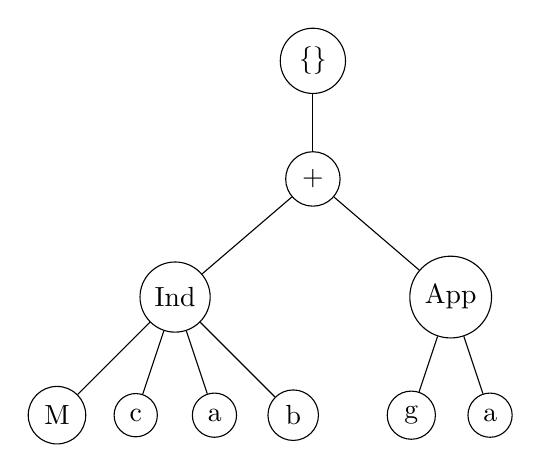
\begin{tikzpicture}[
		    auto,
		    level 1/.style={sibling distance=45mm},
		    level 2/.style={sibling distance=35mm},
		    level 3/.style={sibling distance=10mm}]
		    \node [circle,draw] (z){\{\}}
		        child {
		            node[circle,draw] (a) {+}
		            child { 
		                node[circle,draw] (c) {Ind}
		                child {
		                	node[circle,draw] (e) {M}
		                } 
		                child {
		                	node[circle,draw] (f) {c}
		                } 
		                child {
		                	node[circle,draw] (g) {a}
		                } 		                
		                child {
		                	node[circle,draw] (g) {b}
		                } 
		            }
		            child { 
		                node[circle,draw] (d) {App} 
		                child {
		                	node[circle,draw] (h) {g}
		                }
		                child {
		                	node[circle,draw] (i) {a}
		                }
		            }    
		        }
		        ;
		\end{tikzpicture}
		\caption{The syntax tree for the domain iteration \ref{code:example}} 
		\label{fig:syntaxtree_iter} 		
	\end{subfigure}
	\begin{subfigure}{.5\textwidth}
		\centering
		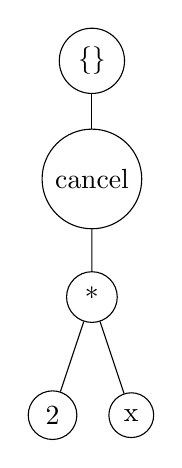
\begin{tikzpicture}[
		    auto,
		    level 1/.style={sibling distance=40mm},
		    level 2/.style={sibling distance=30mm},
		    level 3/.style={sibling distance=10mm}]
			\node [circle,draw] (z){\{\}}
		        child {
		            node[circle,draw] (a) {cancel}
		            child { 
		                node[circle,draw] (c) {*}
		                child {
		                	node[circle,draw] (e) {2}
		                } 
		                child {
		                	node[circle,draw] (f) {x}
		                } 
		            }  
		        }
		        ;
		\end{tikzpicture}
		\caption{The syntax tree for the function \code{g}.}
		\label{fig:syntaxtree_f} 
	\end{subfigure}
	\caption{Syntax trees for the code specified in \ref{code:example}}
\end{figure}
\begin{figure}[h]
	\begin{align*}
		\mathcal{E} &= \abstsyntax{\{M \lbrack c,a,b\rbrack + g(a)\}} \\
					&= \abstsyntax{M \lbrack c,a,b\rbrack + g(a)} \\
					&= \abstsyntax{M \lbrack c,a,b\rbrack} \cup \abstsyntax{g(a)} \\
					&= \abstsyntax{M} \cup \abstsyntax{c} \cup \abstsyntax{a} \cup \abstsyntax{b} \cup \abstsyntax{g} \cup \abstsyntax{a} \\
					&= \accolade{M} \cup\accolade{c} \cup\accolade{a} \cup\accolade{b} \cup\accolade{g} \cup \abstsyntax{\accolade{\operatorname{cancel} 2*x}} \cup \accolade{a} \\
					&= \accolade{M,c,a,b,g} \cup \abstsyntax{\operatorname{cancel} 2*x} \\
					&= \accolade{M,c,a,b,g} \cup \abstsyntax{2*x} \\
					&= \accolade{M,c,a,b,g} \cup \abstsyntax{2} \cup \abstsyntax{x} \\
					&= \accolade{M,c,a,b,g} \cup \emptyset \cup \accolade{x} \\
					&= \accolade{M,c,a,b,g,x}
	\end{align*}
	\caption{Computation of the set $\mathcal{E}$ of all needed identifiers} 
\end{figure}
\newpage



%%%%%%%%%%%%%%%%%%%%%%%%%%%%%%%%%%%%%%%%%%%%%%%%%%%%%%%%%%%
\section{Generation of Host Code}
\label{ex:generated_code}
This section illustrates the process of code generation for the host side, as described in section \ref{sect:compiler_code} with the domain iteration \ref{code:example} with the following listing. The listing shows the code the compiler generates from the function \code{f} specified in section \ref{sect:appendix_funky_full}. The code is slightly edited to make it more readable. \\
\lstinputlisting[language=c++, firstline=8, lastline=66, frame=single]{code/exampleDomain.cpp}
\newpage



%%%%%%%%%%%%%%%%%%%%%%%%%%%%%%%%%%%%%%%%%%%%%%%%%%%%%%%%%%%
\section{Generation of GPU Code}
\label{ex:generated_code_gpu}
This section illustrates the process of code generation for the GPU side, as described in section \ref{sect:compiler_gpu}, using the domain iteration \ref{code:example} with the following listing. The listing shows code the OpenCL kernel the compiler generates from the domain iteration expression body in function \code{f} specified in section \ref{sect:appendix_funky_full}, with a slightly edited layout to make it fit the page. \\
\lstinputlisting[language=c, frame=single, morekeywords={__kernel, __global}]{code/exampleKernel.cl}
\newpage



%%%%%%%%%%%%%%%%%%%%%%%%%%%%%%%%%%%%%%%%%%%%%%%%%%%%%%%%%%%
\section{Function dependencies}
\label{ex:callgraph}
In this section the dependencies between functions will be illustrated. Consider the following example: \\
\lstinputlisting[frame=single, morekeywords={cancel, int, new, domain, public, static, class, inout, unique, finally}, tabsize=2]{code/callgraph.funky} 

This listing can be translated into the call graph given in figure \ref{fig:callgraph}. The graph does not contain any cycles, that means that a topological order exists. It looks as follows: $L=\bracket{h,g,f,d,b,a}$. \\

\begin{figure}
	\begin{tikzpicture}[->,>=stealth',shorten >=1pt,auto,node distance=2.8cm,
	                    semithick]
		\tikzstyle{state H}=[fill=gray]

		\node[initial,state] (M)                    {$kernel$};
		\node[state]         (A) [right of=M] 		{$a$};
		\node[state]         (B) [below of=A] 		{$b$};
		\node[state]         (D) [below right of=B] {$d$};
		\node[state]         (F) [above right of=B]	{$f$};
		\node[state]         (G) [right of=F]       {$g$};
		\node[state]         (H) [below right of=G] {$h$};
		\path (M) edge              	node {a(c)} (A)
		    (A) edge              	node {b(...)} (B)
		        edge              	node {f(i),...} (F)
		    (B) edge [bend right]  	node {d(...)} (D)
		    (D) edge 		 		node {f(2i),...} (F)
		    	edge [bend right]	node {g(3i)} (G)
		    (F) edge 			  	node {g(3i)} (G)
		    (G) edge 			  	node {h(5)} (H);
	\end{tikzpicture}
	\caption{Callgraph of the code listing given in section \ref{ex:callgraph}}
   	\label{fig:callgraph}
\end{figure}